
\subsection{Use Case Diagram}
\begin{figure}[h]
    \centering
    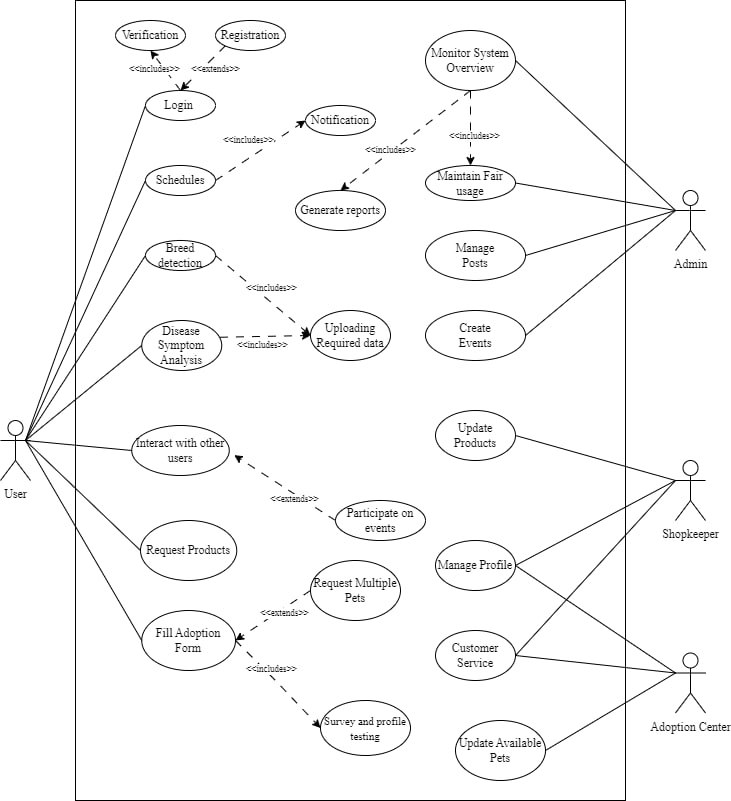
\includegraphics[width= 6in ]{img/use_case.jpg}
    \caption{{Use Case Diagram}}
    \label{fig:use-case}
\end{figure}
\justify
\textbf{User}
\begin{itemize}
    \item \textbf{Verification and Registration:} Users can create accounts, ensuring a secure and verified community.
    \item \textbf{Schedules}: HelloPet assists users in managing pet-related schedules, such as feeding times, veterinary appointments, and play sessions. 
    \item \textbf{Breed Detection:} Users can utilize a breed detection feature to identify the specific breeds of their pets, enhancing their understanding and care.
    \item \textbf{Disease Symptom Analysis:} HelloPet incorporates a symptom analysis tool to help users identify potential health issues in their pets.
    \item \textbf{Interact with Other Users:} Users can connect with fellow pet enthusiasts, fostering a sense of community and providing a platform for sharing experiences and advice.
\end{itemize}
\textbf{Admin}

\begin{itemize}
    \item \textbf{Maintain Fair Usage:} Administrators can enforce fair usage policies, ensuring a positive and secure environment for all users.
    \item \textbf{Monitor System Overview:} Admins have access to a comprehensive system overview, allowing them to track user activities, system performance, and overall engagement.

    \item \textbf{Manage Posts:} Administrators can moderate and manage user-generated content, ensuring that the platform remains a valuable and respectful space.

    \item \textbf{System Monitoring:} Regular monitoring of the system allows administrators to identify potential issues promptly and implement necessary updates or improvements.

\end{itemize}

\textbf{Shopkeeper}
\begin{itemize}
    \item \textbf{Update Products:} Shopkeepers can easily update their product listings, ensuring that users have access to the latest and most relevant pet supplies.

    \item \textbf{Manage Profile:} Shopkeepers can personalize their profiles, providing users with information about their stores and establishing a sense of trust.

    \item\textbf{Customer Service} Shopkeepers can directly engage with users, addressing inquiries, offering recommendations, and providing excellent customer service. 
\end{itemize}


\textbf{Adoption Center}
\begin{itemize}
    \item \textbf{Customer Service:} Adoption centers can offer customer support to users interested in adopting pets, guiding them through the process and answering queries.
    \item \textbf{Manage Profile} Adoption centers can maintain an up-to-date profile, showcasing available pets and providing essential information about their facilities.
    \item \textbf{Update Available Pets} Adoption centers can easily update the list of available pets, ensuring that users have access to the latest information when making adoption decisions.
\end{itemize}